\documentclass{pracamgr}

%%% imports section
\usepackage[polish]{babel}
\RequirePackage{longtable}
\usepackage[T1]{fontenc}
\usepackage[utf8]{inputenc}
\usepackage[pdftex]{color,graphicx}
\usepackage{wrapfig}


\author{Michał Ziemba}

\nralbumu{237954}

\title{Serwis Submit++}

\tytulang{The Submit++ service}

\kierunek{Informatyka}

\opiekun{dr Aleksy Schubert\\
  Instytut Informatyki\\
  }

\date{Czerwiec 2012}

\dziedzina{ 
11.3 Informatyka
}

\klasyfikacja{D. Software}

\keywords{Serwis, zadanie, rozwiązanie, MIMUW}

\begin{document}
\maketitle

\begin{abstract}
  W~pracy przedstawiono opis i dokumentację narzędzia JBSC, służącego do
  analizy statycznej bajtkodu Javy. Jest to wtyczka do środowiska programistycznego
  Eclipse, korzystająca z frameworku Umbra. Umożliwia proste wykrywanie potencjalnie
  niebezpiecznych konstrukcji w kodzie bez jego uruchamiania.
\end{abstract}

\tableofcontents

\chapter*{Wprowadzenie}
\addcontentsline{toc}{chapter}{Wprowadzenie}

    Analiza statyczna kodu polega na badaniu własności programu bez jego uruchamiania,
    w przecwieństwie do analizy dynamicznej. 

    Motywacja
    Ogólnie pojęta analiza statyczna ma coraz większe zastosowanie w procesie wytwarzania wolnego od błędów
    i bezpiecznego kodu. Analiza statyczna kodu wykonywalnego ma zastosowanie w systemach osadzonych, gdzie
    nie ma dostępu do źródeł. Także w przypadku systemów których źródła nie są po prostu wolnodostępne.

Dłuższy opis działania
Java Bytecode Static Checker jest wtyczką do Eclipsa 

%%% TODO Opis rozdziałów

\chapter{Podstawowe pojęcia}\label{r:pojecia}

%%% TODO

\chapter{Kod bajtowy}\label{r:bytecode}
    
    \section{Wprowadzenie}
    Kod bajtowy (\textit{Java Byte Code}) jest formą instrukcji, wykonywanych przez maszynę wirtualną Javy. Programy napisane w języku Java
    są kompilowane do przenośnego kodu, przeważnie w postaci plików \textit{.class}. Zadaniem maszyny wirtualnej
    jest dostarczenie środowiska, umożliwiającego uruchamianie takiego kodu. Maszyna wirtualna, wczytując plik zawierający ciąg bajtów, dostaje kod bajtowy dla wszysztkich metod
    w danej klasie, przechowuje je i uruchamia, gdy konkretna metoda tej klasy zostanie wywołana.
    \begin{wrapfigure}{r}{8cm} % "placement and width parameter for the width of the image space.
        \centering
        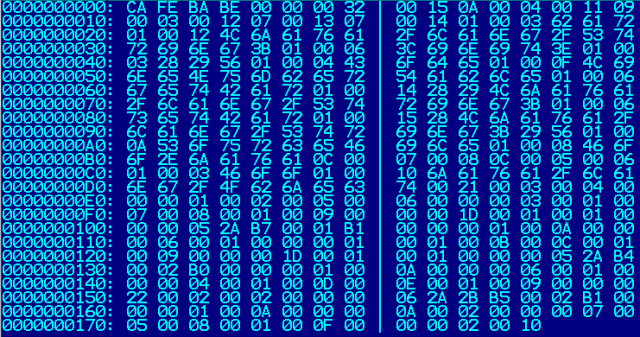
\includegraphics[width=200px]{images/class-hex.png} 
        \caption{Selbstgebaute „Bluesniper“ um Bluetooth-Geräte aus über 1 km Entfernung anzugreifen. (Stand: 2004)}
        \label{bluesniper}
    \end{wrapfigure}
    \begin{center}
        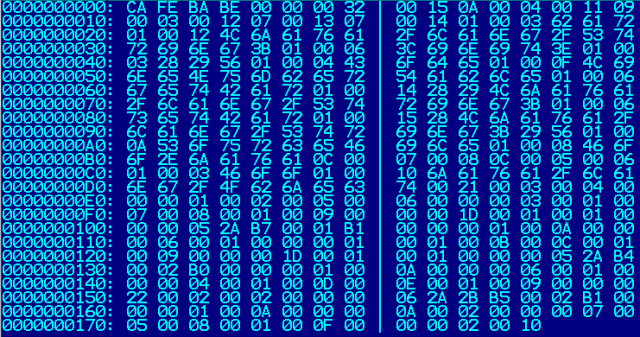
\includegraphics[width=200px]{images/class-hex.png}    
    \end{center}
    Każdy kod instrukcji (ang. \textit{opcode}) ma długość jednego bajta, przy czym niektóre instrukcje wymagają parametrów.
    Każdemu kodowi odpowiada pewne znaczenie (\textit{mnemonic}), przypisane w specyfikacji
    maszyny wirtualnej (zob.~\cite{vmspec})
    %%% TODO dopracować opis

    Na przykład dla ciągu bajtów: 03 3b 84 00 01 1a 05 68 3b a7 ff f9
    Otrzymujemy po deassemblacji:
    \begin{center}
        \begin{tabular}{rr}
            mnemonic & corresponding codes \\
            iconst\_0 & 03 \\
            istore\_0 & 3b \\
            iinc 0, 1 & 84 00 01 \\
            iload\_0 & 1a \\
            iconst\_2 & 05 \\
            imul & 68 \\
            istore\_0 & 3b \\
            goto $-7$ & a7 ff f9 \\
        \end{tabular}
    \end{center}

    Ponieważ maszyna wirualna Javy nie posiada rejestrów, większość operacji używa stosu do przechowywania wartości.
    %%% TODO opis stosu i operacji na nim

    \section{Opis bajtkodu}
    Specjalne i zarezerwowane instrukcje:
    \begin{itemize}
        \item 
        \item
    \end{itemize}
    
    Instrukcje kodu bajtowego można podzielić na następujące grupy:
    \begin{itemize}
        \item
    \end{itemize}
    
    Wyróżniamy podstawowe typy, na których operują instrukcje:
    \begin{center}
        \begin{tabular}{rrr}
            oznaczenie & typ & definicja \\
            b & byte    & one-byte signed two's complement integer \\
            si & short   & two-byte signed two's complement integer \\
            i & int     & 4-byte signed two's complement integer \\
            l & long    & 8-byte signed two's complement integer \\
            f & float   & 4-byte IEEE 754 single-precision float \\
            d & double  & 8-byte IEEE 754 double-precision float \\
            c & char    & 2-byte unsigned Unicode character \\
        \end{tabular}
    \end{center}
    
    Każda instrukcja określa, jakiego typu jest argument, zatem sama maszyna wirtualna nie musi znać typów
    samych wartości, po prostu przekazywane one są jako ciąg bajtów, w porządku \textit{big-endian}, na przykład:
    ciąg bajtów: 17 01 00
    odpowiada:   sipush 256;      // 17 01 00
    
    \section{Struktura pliku \textit{.class}}
    %%% TODO opis pliku class: http://www.vijaymukhi.com/vmis/classprj.htm
    Constants pool
    
    \section{Przykład generowania kodu bajtowego}
    Dla prostego programu w języku Java:
    \begin{verbatim}
    public class HelloWorld {
        public static void main(String[] args) {
            System.out.println("Hello, world!");
        }
    }
    \end{verbatim}
    kod bajtowy wygenerowany przy pomocy deasemblacji (polecenie $java -d$) wygląda następująco:
    \begin{verbatim}
    Compiled from "HelloWorld.java"
public class HelloWorld extends java.lang.Object
 SourceFile: "HelloWorld.java"
 minor version: 0
 major version: 50

{
public HelloWorld();
 Code:
  Stack=1, Locals=1, Args_size=1
  0: aload_0
  1: invokespecial #1; //Method java/lang/Object."<init>":()V
  4: return

 LineNumberTable:
  line 1: 0

public static void main(java.lang.String[]);
 Code:
  Stack=2, Locals=1, Args_size=1
  0: getstatic #2; //Field java/lang/System.out:Ljava/io/PrintStream;
  3: ldc #3; //String Hello, world!
  5: invokevirtual #4; //Method java/io/PrintStream.println:(Ljava/lang/String;)V
  8: return
 LineNumberTable:
  line 5: 0
  line 6: 8
}
    \end{verbatim}
    
    %%% TODO Przykład kodu bajtowego?

\chapter{Analiza statyczna}\label{r:staticanalysis}

    Analiza statyczna polega na badaniu kodu źródłowego bez jego uruchamiania. Pozwala wykryć potencjalnie
    niebezpieczne konstrukcje w kodzie. Jednak fakt niewykrycia błędu na poziomie analizy statycznej nie czyni
    kodu bezbłędnym.
    
    Możliwości i ograniczenia (zalety)
    Zalety korzystania z narzędzi do analizy statycznej:
    \begin{itemize}
        \item Sprawdzenia wykonywane przez narzędzie, w odróżnieniu od sprawdzenia programisty,
              pozwalają wykryć potencjalne błędy w miejscach mniej interesujących, które mogły zostać pominięte
              lub przeoczone przez programistę.
        \item Analiza statyczna daje możliwość wykrycia problemów u ich źródła. Pozwala uniknąć sytuacji,
              kiedy w trakcie uruchamiania programu otrzymujemy błąd przepełnienia buforu, a nie wiemy dokładnie
              kiedy, gdzie i dlaczego to przepełnienie nastąpiło.
        \item Błędy są znajdowane na wczesnym etapie rozwijania kodu. To daje możliwość uniknięcia być może
              kosztownego usuwania tego błędu na późniejszym etapie.
    \end{itemize}
    
    Najpoważniejszym zarzutem, który pojawia się pod adresem narzędzi do analizy statycznej jest fakt, że
    produkują zbyt wiele ostrzeżeń, z których większość jest nieprzydatnych. Takie fałszywe ostrzeżenia nazywamy
    \textit{false negatives}.
    
    Zakres analizy statycznej
    Przy pomocy analizy statycznej można wykonywać następujące sprawdzenia:
    \begin{itemize}
        \item 
    \end{itemize}
    
    Etapy analizy
    
    Co można sprawdzać
    
    False positives, false negatives
    
    Przykładowe narzędzia i ch krótki opis:
    \begin{itemize}
        \item lint
        \item findbugs
        \item escjava2
    \end{itemize}
    
    
\chapter{Integracja}\label{r:integration}

    Co to jest Umbra?

    Połączenie z frameworkiem Umbra

\chapter{Funkcjonalność systemu}\label{r:funkcjonalnosc}

\section{Wprowadzenie}


\chapter{Środowisko systemu}\label{r:srodowisko}

\section{Serwer}


\chapter{Budowa systemu}\label{r:budowa}

\section{Architektura systemu}




\chapter{Podsumowanie}\label{r:podsumowanie}


\appendix

\chapter{Listingi kodu bajtowego}

%%% TODO

\chapter{Dostarczone dokumenty}

Obiekty dostarczone w ramach pracy licencjackiej to:
\begin{itemize}
\item dokument z treścią pracy licencjackiej
\item płyta CD
\end{itemize}

\chapter{Spis zawartości płyty CD}




\begin{thebibliography}{99}
\addcontentsline{toc}{chapter}{Bibliografia}

\bibitem[JVMSpec]{vmspec} \url{''http://docs.oracle.com/javase/specs/jvms/se7/html/index.html''}.

\bibitem[Fif01]{ff-sr} Filigran Fifak, \textit{O fetorach
    $\sigma$-$\rho$}, Acta Fetorica, 2001.

\end{thebibliography}


\end{document}

